\begin{theorem} (Полнота $\cL(E_1, E_2)$ относительно поточечной сходимости)
	Пусть $E_1, E_2$ --- банаховы пространства, $\{A_n\}_{n = 1}^\infty \subseteq \cL(E_1, E_2)$. Если для любого $x \in E_1$ последовательность $\{A_nx\}_{n = 1}^\infty$ фундаментальна в $E_2$, то существует такой оператор $A \in \cL(E_1, E_2)$, что $A_n$ сходятся поточечно к $A$.
\end{theorem}

\begin{proof}
	Зафиксируем $x \in E_1$. Раз $\{A_nx\}_{n = 1}^\infty \subseteq E_2$ фундаментальна, то у неё есть предел (за счёт банаховости $E_2$). Положим значение оператора $A$ по определению этим пределом:
	\[
		Ax := \lim_{n \to \infty} A_nx
	\]
	Покажем, что определённый таким образом оператор принадлежит $\cL(E_1, E_2)$:
	\begin{itemize}
		\item $A$ линеен. Это на самом деле так, в силу линейности предела и $A_n$:
		\[
			\forall \alpha, \beta \in \K, a, b \in E_1\ \ A(\alpha a + \beta b) = \lim_{n \to \infty} A_n(\alpha a + \beta b) = \alpha \lim_{n \to \infty} A_na + \beta \lim_{n \to \infty} A_nb = \alpha Aa + \beta Ab
		\]
		
		\item $A$ ограничен. Мы хотим проделать те же действия, что и при доказательстве обычной полноты $\cL(E_1, E_2)$. Коль скоро $\lim_{n \to \infty} \|A_nx\| = \|Ax\|$, то последовательность норм $\{\|A_nx\|\}_{n = 1}^\infty$ ограничена при любом $x$, а значит по теореме Банаха-Штейнгауза-Хана должна быть ограничена последовательность норм операторов $\{\|A_n\|\}_{n = 1}^\infty$. Если обозначить константу ограничения за $M > 0$, то мы получаем знакомое предельное неравенство:
		\[
			\forall n \in \N\ \ \forall x \in E_1\ \|A_nx\| \le M\|x\| \Lora \|Ax\| \le M\|x\|
		\]
	\end{itemize}
\end{proof}

\begin{note}
	Поточечная сходимость операторов $A_n \in \cL(E_1, E_2)$ не влечёт за собой сходимость непосредственно операторов по норме $\lim_{n \to \infty} A_n = A$. Контрпример достаточно просто увидеть в пространстве $\ell_2$. Определим $A_n$ как срезку аргумента:
	\[
		A_nx = (x_1, \ldots, x_n, 0, \ldots)
	\]
	Стало быть, при каждом фиксированном $x \in \ell_2$ есть предел $\lim_{n \to \infty} A_nx = Ix = x$. Однако совершенно понятно, что $\lim_{n \to \infty} \|A_n - I\| \neq 0$, ибо всегда можно подобрать <<ломающий>> $x$, у которого есть единичная координата в позиции больше $n$.
\end{note}

\begin{theorem} (Критерий поточечной сходимости последовательности линейных ограниченных операторов)
	Пусть $E_1$ --- банахово пространство, $\{A_n\}_{n = 1}^\infty \subseteq \cL(E_1, E_2)$ --- последовательность линейных ограниченных операторов, $A \in \cL(E_1, E_2)$. Тогда $A_n$ поточечно сходятся к $A$ тогда и только тогда, когда выполнено 2 условия:
	\begin{itemize}
		\item Последовательность норм $\{\|A_n\|\}_{n = 1}^\infty$ ограничена
		
		\item $\exists Y \subseteq E_1 \colon \cl [Y] = E_1 \wedge \forall y \in Y\ \lim_{n \to \infty} A_ny = Ay$
	\end{itemize}
\end{theorem}

\begin{anote}
	Критерий немного напоминает аналогичные критерии независимости сигма-алгебр в теории вероятностей. С маленьким условием на сами операторы и с наличием хорошего множества $Y$ мы умеем распространять сходимость на всё пространство.
\end{anote}

\begin{proof}~
	\begin{itemize}
		\item[$\Ra$] Коль скоро есть поточечная сходимость, то в каждой точке $x \in E_1$ последовательность норм $\{\|A_nx\|\}_{n = 1}^\infty$ ограничена. Стало быть, по теореме Банаха-Штейнгауза-Хана последовательность норм операторов ограничена. За $Y$ мы можем смело взять $E_1$ и не думать вообще.
		
		\item[$\La$] Рассмотрим $x \in E_1$. За счёт существования всюду плотного $[Y]$, мы можем всегда найти близкую точку из $Y$ для $x$:
		\[
			\forall \eps > 0\ \exists y \in [Y] \such \|x - y\| < \eps
		\]
		Показывать сходимость будем через оценку нормы разности $A_nx - Ax$ при помощи неравенства треугольника:
		\[
			\|A_nx - Ax\| \le \|A_nx - A_ny\| + \|A_ny - Ay\| + \|Ay - Ax\|
		\]
		Разберёмся с каждым слагаемым отдельно (далее $M > 0$ --- это константа ограничения последовательности норм):
		\begin{itemize}
			\item $\|A_nx - A_ny\| \le \|A_n\| \cdot \|x - y\| < M \eps$
			
			\item $A_ny - Ay = (A_n - A)y$. Коль скоро на $Y$ операторы $A_n$ сходятся поточечно к $A$, то есть поточечная сходимость к любой точке $y \in [Y]$ (ибо это конечная линейная комбинация точек из $Y$). Стало быть:
			\[
				\forall y \in [Y]\ \forall \eps > 0\ \exists N \in \N \such \forall n \ge N\ \ \|A_ny - Ay\| < \eps
			\]
			
			\item $\|Ay - Ax\| \le \|A\| \cdot \|y - x\| < \|A\|\eps$
		\end{itemize}
		Итого:
		\[
			\forall \eps > 0\ \exists N \in \N \such \forall n \ge N\ \ \|A_nx - Ax\| \le (M + 1 + \|A\|)\eps
		\]
		Это напрямую означает поточечную сходимость $A_n$ к $A$.
	\end{itemize}
\end{proof}

\begin{corollary}
	Если в условиях последней теоремы $\{A_n\}_{n = 1}^\infty$ сходятся на $Y$ не просто поточечно, а по норме операторов, то в теореме можно не требовать от $A$ быть заранее линейным ограниченным оператором.
\end{corollary}

\begin{proof} (теоремы \ref{op_cont_th})
	\begin{enumerate}
		\item (Идея) Пусть $\wdt{A}$ --- некоторое продолжение оператора $A$ по условию теоремы. Тогда несложно заметить, что по условию выполнено утверждение:
		\[
		\forall x \in E_1\ \exists \{x_n\}_{n = 1}^\infty \subseteq D(A) \such \lim_{n \to \infty} x_n = x \wedge \wdt{A}x_n = Ax_n \xrightarrow[n \to \infty]{} \wdt{A}x
		\]
		Стало быть, нужно отталкиваться от поточечного определения $\wdt{A}$.
		
		\item (Существование) Определим $\wdt{A}$ согласно идее (оператор $A$ непрерывен, поэтому пределы всегда есть):
		\[
		\forall x \in E_1\ \forall \{x_n\}_{n = 1}^\infty \subseteq D(A) \such \lim_{n \to \infty} x_n = x \Ra \wdt{A}x := \lim_{n \to \infty} Ax_n
		\]
		Теперь, покажем корректность такого определения:
		\begin{itemize}
			\item Значение $\wdt{A}$ не зависит от рассматриваемой последовательности $\{x_n\}_{n = 1}^\infty \subseteq D(A)$, $\lim_{n \to \infty} x_n = x$. Действительно, рассмотрим 2 последовательности $\lim_{n \to \infty} x_{n, 1} = \lim_{n \to \infty} x_{n, 2} = x$. Тогда, можно написать следующее неравенство:
			\[
			\|Ax_{1, n} - Ax_{2, m}\| \le \|A\| \cdot \|x_{1, n} - x_{2, m}\| \xrightarrow[n, m \to \infty]{} 0
			\]
			Более строго, нужно поочерёдно устремить в бесконечность $n, m \to \infty$ и тем самым сделать 2 предельных перехода.
			
			\item Почему $\wdt{A}$ --- линейный оператор? Это тривиально из линейности предела:
			\begin{multline*}
			\forall x, y \in E_1,\ \alpha, \beta \in \K\ \ \wdt{A}(\alpha x + \beta y) = \lim_{n \to \infty} A(\alpha x_n + \beta y_n) =
			\\
			\alpha \lim_{n \to \infty} Ax_n + \beta \lim_{n \to \infty} Ay_n = \alpha Ax + \beta Ay
			\end{multline*}
			
			\item Почему $\wdt{A}$ --- ограниченный оператор? Воспользуемся старым добрым предельным переходом:
			\[
			\|\wdt{A}x_n\| = \|Ax_n\| \le \|A\| \cdot \|x_n\| \Ra \|\wdt{A}x\| \le \|A\| \cdot \|x\| \Ra \|\wdt{A}\| \le \|A\|
			\]
			При этом из определения $\wdt{A}$ сразу следует, что $\|\wdt{A}\| \ge \|A\|$. Таким образом, мы сразу установили равенство $\|\wdt{A}\| = \|A\|$
		\end{itemize}
		
		\item (Единственность) Предположим, есть 2 продолжающих оператора: $\wdh{A}$ и $\wdt{A}$. Как мы и требовали, они должны быть согласованы с $A$. Стало быть, можно записать следующее:
		\[
		\forall x \in E_1\ \ \wdh{A}x = \lim_{n \to \infty} Ax_n = \wdt{A}x
		\]
		Следовательно, $\wdh{A} = \wdt{A}$.
	\end{enumerate}
\end{proof}

\subsection*{Применение теоремы Банаха-Штейнгауза}

\begin{problem}
	Вернёмся на семестр назад, в гармонический анализ. Если $f \in C_{2\pi} = CP[-\pi; \pi]$ (Continuous Periodic), то такой функции мы \textit{сопоставляли} ряд Фурье:
	\[
		f \sim \frac{a_0}{2} + \sum_{k = 1}^\infty a_k\cos(kx) + b_k\sin(kx)
	\]
	И мы также изучили условия, при которых этот ряд сходится к $f$. Эту тему мы можем перевести на язык функционального анализа. Пусть $S_n(f, x)$ означает, как и раньше, частичную сумму ряда Фурье. Тогда её можно записать в виде интеграла с ядром Дирихле:
	\[
		S_n(f, x) = \frac{1}{\pi}\int_{-\pi}^\pi D_n(x - t)f(t)dt,\ D_n(t) = \frac{\sin\Big(\ps{n + \frac{1}{2}}t\Big)}{2\sin\frac{t}{2}}
	\]
	Эти частичные суммы можно рассмотреть как оператор $S_n \in \cL(C_{2\pi})$, то есть $S_n$ переводит $f$ в какую-то ещё одну функцию, причём из $C_{2\pi}$. Изучение равномерной сходимости ряда Фурье к функции $f$ это в точности изучение поточечной сходимости операторов $S_n$ к тождественному оператору $I$.
	
	Можно задаться вопросом: а можем ли мы обобщить $S_n$, если рассматривать его как оператор в пространстве $\cL(C_{2\pi})$? Во-первых, можем, а во-вторых, как следствие, мы получим интересное доказательство того факта, что не у всех функций из $C_{2\pi}$ может быть поточечная сходимость ряда Фурье, без построения точного контрпримера!
\end{problem}

\begin{definition}
	Пусть $f \in C[a; b]$, $K \in C\big([a; b]^2\big)$. Тогда \textit{оператором Фредгольма с ядром $K$} называется следующий оператор $A$:
	\[
		\forall x \in [a; b]\ (Af)(x) := \int_a^b K(x, t)f(t)dt
	\]
\end{definition}

\begin{note}
	Далее мы живём в пространстве $C[a; b]$.
\end{note}

\begin{proposition}
	Оператор Фредгольма с ядром $K$ принадлежит к классу $\cL(C[a; b])$.
\end{proposition}

\begin{proof}
	Линейность и непрерывность получаются в силу свойств интеграла (второе следует из интегрирования непрерывной функции).
\end{proof}

\begin{proposition}
	Если $A$ --- оператор Фредгольма с ядром $K$, то норму оператора можно найти явно:
	\[
		\|A\| = \max_{x \in [a; b]} \int_a^b |K(x, t)|dt
	\]
\end{proposition}

\begin{proof}~
	\begin{itemize}
		\item[$\le$] В эту сторону показать неравенство крайне просто:
		\begin{multline*}
			\|A\| = \sup_{\|f\| = 1} \|Af\| = \sup_{\|f\| = 1} \max_{x \in [a; b]} \md{\int_a^b K(x, t)f(t)dt} \le
			\\
			\sup_{\|f\| = 1} \max_{x \in [a; b]} \int_a^b |K(x, t)| \cdot |f(t)|dt \le
			\\
			\sup_{\|f\| = 1} \|f\| \cdot \max_{x \in [a; b]} \int_a^b |K(x, t)|dt = \max_{x \in [a; b]} \int_a^b |K(x, t)|dt
		\end{multline*}
		
		\item[$\ge$] Обозначим потенциальное выражение нормы за $M$. По сути нам нужно для любого $\eps > 0$ просто найти $f \in C[a; b]$, $\|f\| = 1$ такую, что $\|Af\| \ge M\eps$. Идея состоит в том, в цепочке неравенств выше у нас лишь одно проблемное место, где просто так равенства не получить --- это переход к модулю под знаком интеграла. Если бы мы мысленно забыли, что нам нужна непрерывная $f$, то мы бы могли взять $f_0(t) = \sgn K(x_0, t)$ и нужные равенства бы соблюлись. Значит, попробуем приближать эту функцию знака, например через линейное сглаживание (считаем, что $x$ фиксирован):
		
		\begin{center}
			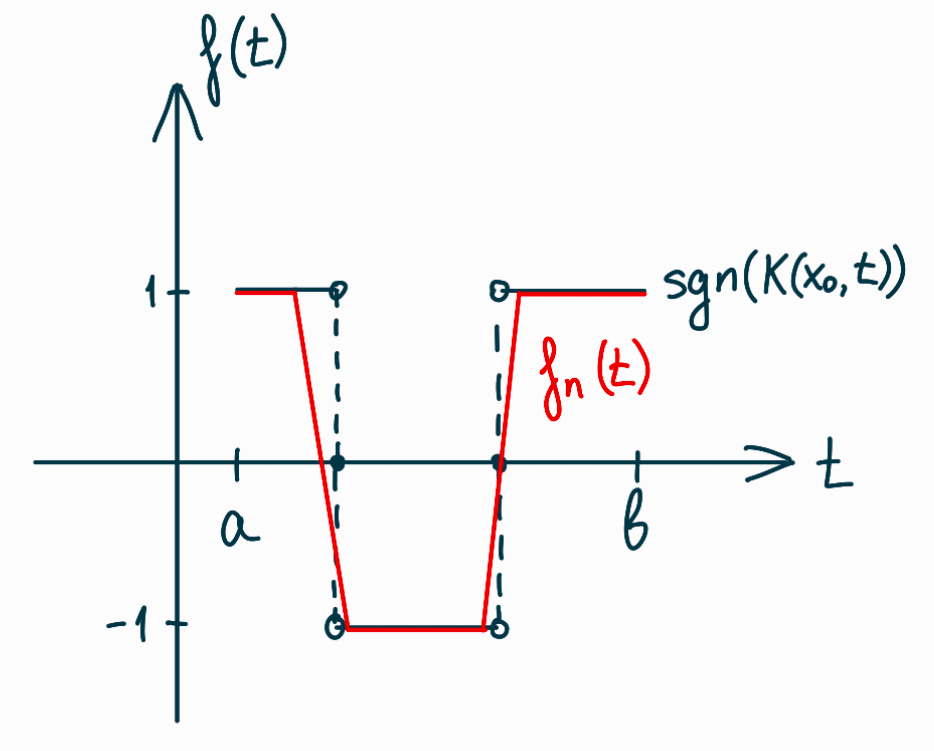
\includegraphics[width=0.4\textwidth]{images/4pic.png}
		\end{center}
		
		Более формально, можно записать так:
		\[
			\forall n \in \N\ \ f_n(t) = \System{
				&{\sgn(K(x, t)), |K(x, t)| \ge \frac{1}{n}}
				\\
				&{linear, |K(x, t)| < \frac{1}{n}}
			}
		\]
		Используя подобную последовательность $f_n$, мы можем оценить снизу норму оператора:
		\begin{multline*}
			\forall n \in \N\ \ \|A\| = \sup_{\|f\| = 1} \|Af\| \ge \|Af_n\| = \max_{x \in [a; b]} \md{\int_a^b K(x, t)f_n(t)dt} \ge
			\\
			\md{\int_a^b K(x_0, t)f_n(t)dt} = \md{\int_{|K(x_0, t)| \ge \frac{1}{n}} K(x_0, t)f_n(t)dt + \int_{|K(x_0, t)| < \frac{1}{n}} K(x_0, t)f_n(t)d\mu(t)} \ge
			\\
			\int_{|K(x_0, t)| \ge \frac{1}{n}} K(x_0, t)f_n(t)dt - \md{\int_{|K(x_0, t)| < \frac{1}{n}} K(x_0, t)f_n(t)d\mu(t)}
		\end{multline*}
		Последний переход сделан при помощи неравенства $||a| - |b|| \le |a - b|$. Второй интеграл стремится к нулю с ростом $n$, поэтому его вклад в модуль можно забыть. При этом же для первого интеграла мы в силу определения $f_n$ имеем право написать следующее:
		\begin{multline*}
			\int_{|K(x_0, t)| \ge \frac{1}{n}} K(x_0, t)f_n(t)dt = \int_{|K(x_0, t)| \ge \frac{1}{n}} |K(x_0, t)|dt =
			\\
			M - \int_{|K(x_0, t)| < \frac{1}{n}} |K(x_0, t)|d\mu(t) \ge M - \frac{b - a}{n}
		\end{multline*}
		Стало быть, с ростом $n$ оценка нормы $\|A\|$ стремится снизу к $M$, что мы и хотели показать.
	\end{itemize}
\end{proof}

\begin{corollary}
	Формула нормы оператора Фредгольма верна и в случае оператора $S_n \in \cL(C_{2\pi})$. Более того, норма этих операторов стремится в бесконечность, то есть $\sup_{n \in \N} \|S_n\| = \infty$
\end{corollary}

\begin{proof}
	Оценим норму $\|S_n\|$ через полученную формулу:
	\begin{multline*}
		\|S_n\| = \frac{1}{\pi} \max_{x \in [-\pi; \pi]} \int_{-\pi}^\pi |D_n(x - t)|dt \ge \frac{1}{\pi} \int_{-\pi}^\pi |D_n(-t)|dt = \frac{2}{\pi} \int_0^\pi \frac{\md{\sin((n + 1 / 2)t)}}{2|\sin \frac{t}{2}|}dt \ge
		\\
		\frac{1}{\pi} \int_0^\pi \frac{|\sin((n + 1 / 2)t)|}{t / 2}dt = [s = (n + 1 / 2)t] = \frac{1}{2\pi} \int_0^{(n + 1 / 2)\pi} \frac{|\sin s|}{s}ds \approx \ln n
	\end{multline*}
	Отсюда $\lim_{n \to \infty} \|S_n\| = \infty$, что и требовалось.
\end{proof}